\documentclass[a4paper,12pt]{article}

\title{addFC -- дополнительные инструменты для FreeCAD}
\author{Голодников Сергей}
\date{\today}

\usepackage[left=2cm,right=2cm,top=2cm,bottom=2cm]{geometry}
\usepackage{fontspec}
\setmainfont{PT Astra Serif}
\usepackage[ddmmyyyy]{datetime}
\renewcommand{\dateseparator}{.}
\usepackage{graphicx}
\usepackage{caption}
\captionsetup[figure]{name=Изображение}
\usepackage[
	pdfauthor={Golodnikov Sergey},
	pdftitle={Additional tools for FreeCAD},
	pdfsubject={addFC},
	colorlinks=true,
	linkcolor=blue]{hyperref}




\begin{document}
\maketitle




\section{Цели и задачи}

\begin{itemize}
	\item Спецификация материалов -- BOM.
	\item Пакетная обработка деталей из листового металла.
	\item Создание конструкторской документации.
	\item Автоматизация процессов.\\
\end{itemize}

Главная задача верстака -- упростить работу с большими и «сложными» сборками, в особенности со сборками содержащими детали из листового металла.

«Сложными» я называю параметрические модели (сборки) с большим количеством объектов и узлов в виде ссылок и связей (App::Link).

Основной смысл в повторном использовании компонентов.

\begin{figure}[htp]
	\centering
	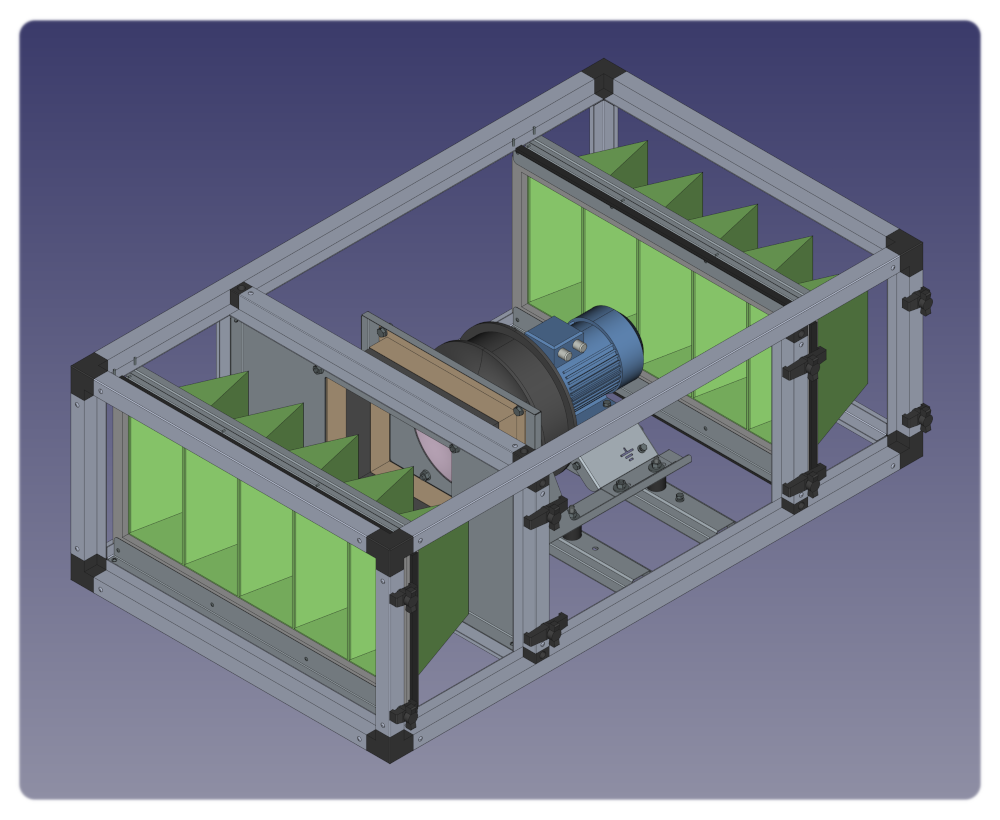
\includegraphics[scale=0.48]{img/assembly_example.png}
	\caption{Пример «сложной» сборки}
	\label{sec:assembly_example}
\end{figure}

\begin{center}\emph{Логика работы базируется на добавлении пользовательских свойств к объектам, придавая им определённые смысловые значения.}\end{center}

% section end




\section{Панель инструментов}

При выборе верстака \textbf{addFC} станет доступна панель его инструментов, выглядит она так:

\begin{figure}[htp]
	\centering
	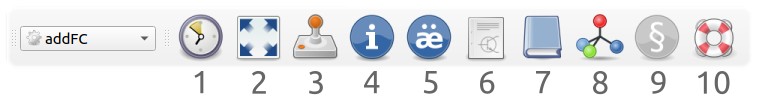
\includegraphics[scale=0.8]{img/toolbar.png}
	\caption{Панель инструментов}
	\label{sec:toolbar}
\end{figure}

\begin{flushleft}Инструменты по порядку:\end{flushleft}
\begin{enumerate}
	\item Открыть последний рабочий файл -- \textbf{Recent File} (Alt+Shift+R).\label{sec:1}
	\item Изометрический вид и отображение в размер окна -- \textbf{Display} (Alt+Shift+D).\label{sec:2}
	\item Управление моделью -- \textbf{Model Control} (Alt+Shift+C).\label{sec:3}
	\item Спецификация материалов, BOM -- \textbf{Specification} (Alt+Shift+S).\label{sec:4}
	\item Наполнение объекта свойствами -- \textbf{Add Properties} (Alt+Shift+A).\label{sec:5}
	\item Создание трубопровода по координатам -- \textbf{Pipe} (Alt+Shift+P).\label{sec:6}
	\item Вид с разнесёнными частями -- \textbf{Explode} (Alt+Shift+E).\label{sec:7}
	\item Создать чертёж на основе шаблона -- \textbf{Creating a Drawing} (Alt+Shift+I).\label{sec:8}
	\item Помощь и примеры -- \textbf{Help and Examples}.\label{sec:9}
\end{enumerate}

Примечание: FreeCAD позволяет создавать дополнительные панели инструментов, рекомендую воспользоваться этим и создать из наиболее востребованных функций собственную панель для отображения её на своём основном рабочем верстаке, например в PartDesign.

% section end
\pagebreak




\section{Помощь и примеры}

В составе верстака есть образцы изучив которые можно лучше понять принципы его работы, чтобы открыть один из них -- воспользуйтесь командой \hyperref[sec:9]{Help and Examples} на панели инструментов. Наиболее подходящий пример -- \textbf{Assembly}, он и будет рассмотрен в данном руководстве.

\begin{figure}[htp]
	\centering
	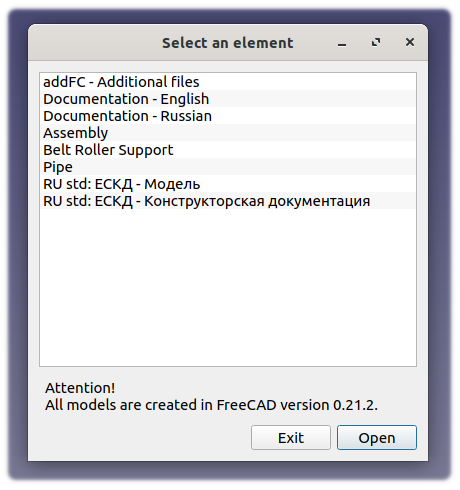
\includegraphics[scale=1]{img/assistant.png}
	\caption{Помощь и примеры}
	\label{sec:assistant}
\end{figure}

\begin{itemize}
	\item \textbf{Additional files} -- дополнительные файлы, такие как шаблоны чертежей и шрифты.
	\item \textbf{Documentation} -- документация по работе с верстаком.
	\item \textbf{Assembly} и \textbf{Belt Roller Support} -- примеры моделей (сборок) и работы со свойствами.\\Assembly -- модель параметрическая.
	\item \textbf{Pipe} -- пример использования инструмента \hyperref[sec:6]{Pipe}.
	\item \textbf{RU std: ЕСКД} -- оформление конструкторской документации по стандартам,\\включая автоматическую генерацию спецификации.
\end{itemize}

% section end
\pagebreak




\section{Параметры и настройки}

\begin{figure}[htp]
	\centering
	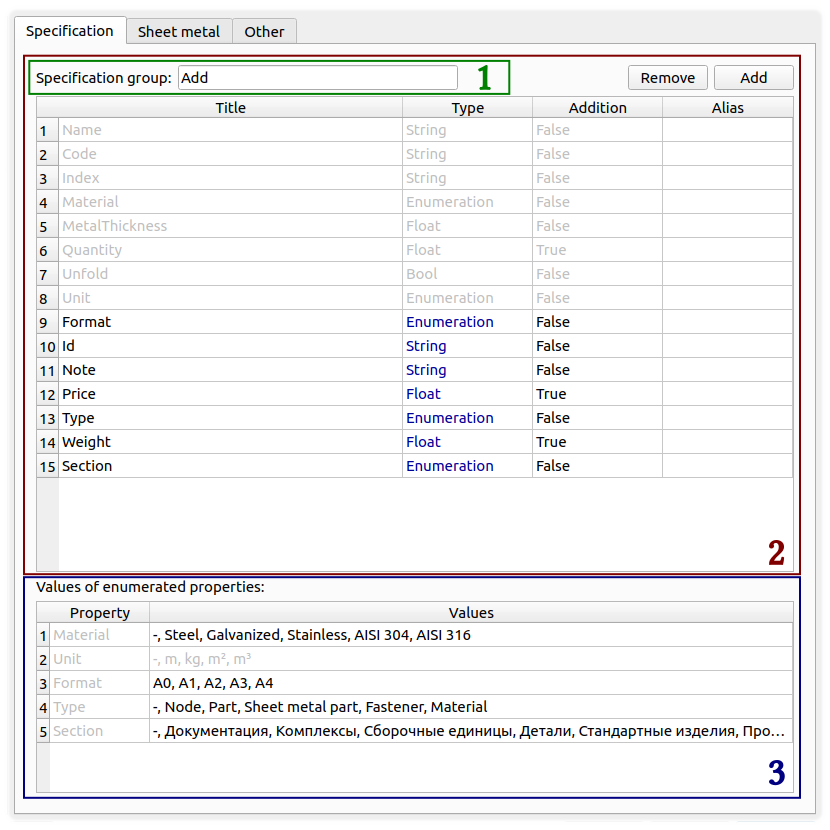
\includegraphics[width=1\textwidth]{img/pref_specification.png}
	\caption{Параметры спецификации}
	\label{sec:pref_specification}
\end{figure}

\subsection{Область 1 -- Наименование для группировки свойств}
Свойства, которые мы добавим объектам будут объединены в специальную группу, наименование которой можно указать в соответствующем поле. Это облегчит визуальное восприятие и не позволит нашим свойствам смешиваться со стандартными.


\pagebreak


\subsection{Область 2 -- Свойства пользователя}

В данной таблице находятся все доступные для использования свойства.
\begin{itemize}
	\item \textbf{Title} -- наименование свойства (важно: только латинские символы).
	\item \textbf{Type} -- тип значения свойства, для использования доступны:
	\begin{itemize}
		\item \textbf{Bool} -- логический тип данных (true или false).
		\item \textbf{Enumeration} -- список из заранее заданных значений.
		\item \textbf{Float} -- число с плавающей точкой.
		\item \textbf{Integer} -- целое число.
		\item \textbf{String} -- текстовая строка.
	\end{itemize}
	\item \textbf{Addition} -- указывает на необходимость суммировать все значения свойства\\(пример использования: общая масса сборки).
	\item \textbf{Alias} -- псевдоним свойства, значение которое заменит \textbf{Title} при показе или\\ экспорте спецификации (позволяет обойти ограничение на латинские символы).
\end{itemize}

\begin{flushleft}Кнопки \textbf{Remove} и \textbf{Add} соответственно позволяют удалить выделенное в таблице свойство или добавить строку для создания нового.\end{flushleft}

\subsection{Область 3 -- Списки заранее заданных значений}
Все свойства с типом данных \textbf{Enumeration} отображаются в этой области.\\В колонке \textbf{Values} -- разделённые запятой значения для формирования списка.

% section end




\section{Свойства объектов}

Неактивные свойства и значения в таблице, являются основными и требуются для корректной работы верстака.

\begin{center}\emph{Свойства должны придать смысловую нагрузку объектам FreeCAD.}\end{center}

\begin{itemize}
	\item \textbf{Name} -- имя, наименование объекта -- самое важное свойство, программа работает с элементами только при условии наличия у них имени. Наименование должно отражать суть объекта.
	\item \textbf{Code} -- кодовое обозначение элемента или детали.
	\item \textbf{Index} -- идентификатор для определения позиции объекта в сборке.
	\item \textbf{Material} -- материал объекта (список значений). Для листового металла это важное свойство, при создании плоского вида детали (развёртка) для оцинкованной и нержавеющей стали используются разные коэффициенты, также это свойство учитывается при сохранении развёртки во внешний файл.
	\item \textbf{MetalThickness} -- толщина металла, краткое обозначение: \textbf{MT}.
	\item \textbf{Unfold} -- определяет необходимость создания плоского вида для конкретного объекта (актуально только для деталей из листового металла).
	\item \textbf{Quantity} и \textbf{Unit} -- количество и единица измерения \textbf{(-, m, kg, m², m³)}. Для штучных элементов значение по умолчанию в большинстве случаев -- это единица \textbf{(-)}. Для различных материалов доступны любые комбинации: например длина уплотнителя \textbf{1,2 m} или количество утеплителя \textbf{4,2 m²}. Важно: значения суммируются для одинаковых по наименованию объектов.
\end{itemize}


\subsection{Дополнительные свойства}

Эти свойства не являются основными (\emph{их можно удалить}), но тем не менее они полезны в работе:
\begin{itemize}
	\item \textbf{Format} -- формат на котором выполнен документ (список значений).
	\item \textbf{Id} -- некий идентификатор объекта для связи с другой программой, например с 1С (код номенклатуры).
	\item \textbf{Note} -- заметка, напоминание или пояснение.
	\item \textbf{Price} -- стоимость объекта.
	\item \textbf{Type} -- тип объекта (список значений). Полезное свойство для группирования элементов при показе или экспорте спецификации.
	\item \textbf{Weight} -- масса объекта.
	\item \textbf{Section} -- разделы спецификации по стандарту ЕСКД.
\end{itemize}

\begin{center}\emph{Для учёта объекта программой, только свойство \textbf{Name} является обязательным, все остальные используются по мере необходимости.}\end{center}

\begin{figure}[htp]
	\centering
	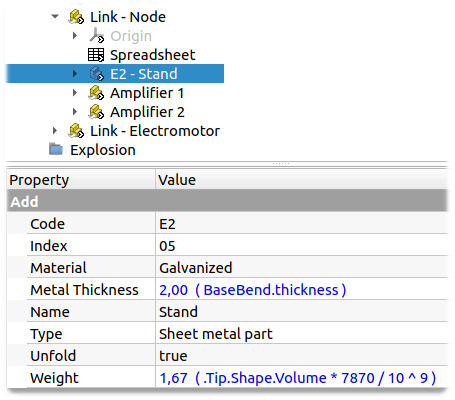
\includegraphics[scale=0.9]{img/properties.png}
	\caption{Пример объекта с заполненными свойствами}
	\label{sec:properties}
\end{figure}


\pagebreak


\begin{figure}[htp]
	\centering
	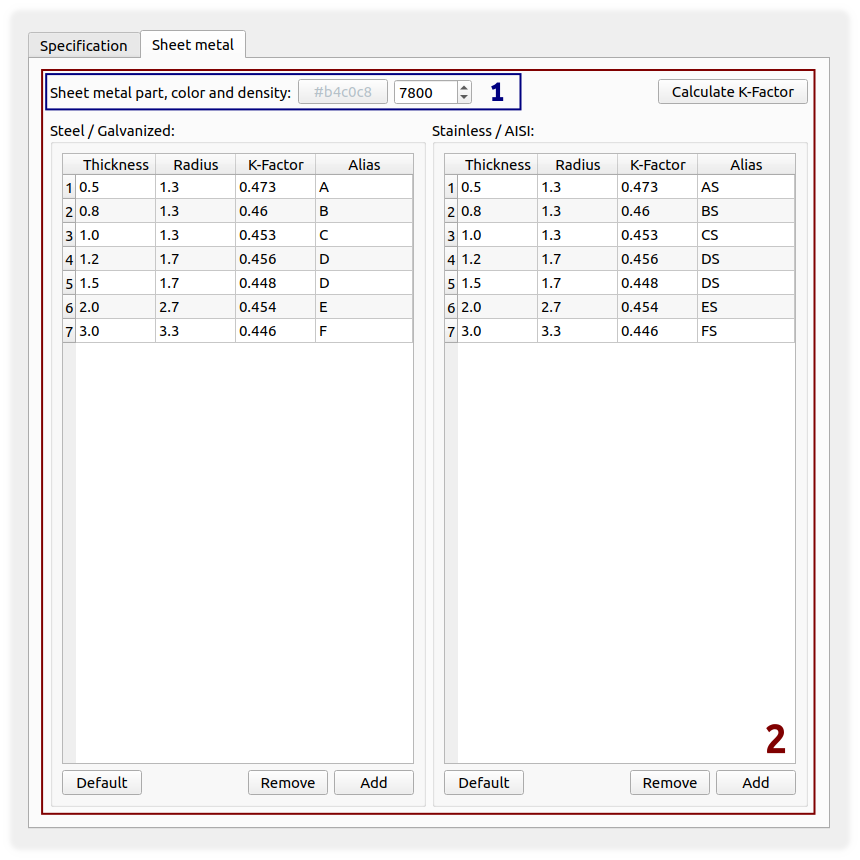
\includegraphics[width=1\textwidth]{img/pref_sm.png}
	\caption{Параметры листового металла}
	\label{sec:pref_sm}
\end{figure}

\subsection{Область 4 -- Параметры для детали из листового металла}
Первое значение -- цвет объекта в формате hex (\verb|#b4c0c8|), второе -- усреднённое значение плотности стали (7800 кг/м³).

\subsection{Область 5 -- Параметры листовой стали}
В этой таблице указаны допустимые для использования толщины (\textbf{thickness}) листового металла и их параметры, такие как внутренний радиус изгиба (\textbf{radius}) и коэффициент К (\textbf{k-factor}) используемый при расчёте плоского вида (развёртки). \textbf{Alias} -- это псевдоним для толщины металла он необходим для корректного экспорта развёрток во внешний формат.\\


\pagebreak


Кнопка \textbf{Calculate K-Factor} автоматически вычисляет коэффициент К (\textbf{k-factor}) для каждой толщины по формулам из сопротивления материалов:

\begin{figure}[htp]
	\centering
	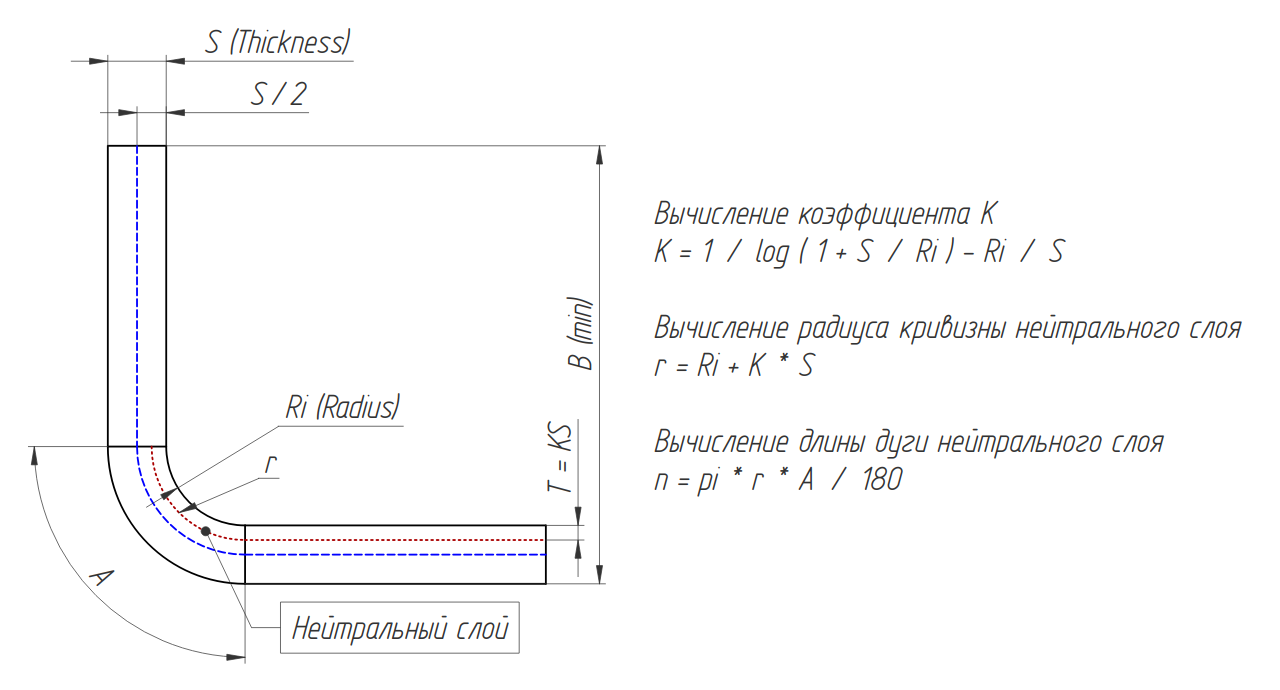
\includegraphics[width=1\textwidth]{img/k_ru.png}
	\caption{Формулы вычислений параметров листового металла}
	\label{sec:k}
\end{figure}

% section end
\pagebreak




\begin{figure}[htp]
	\centering
	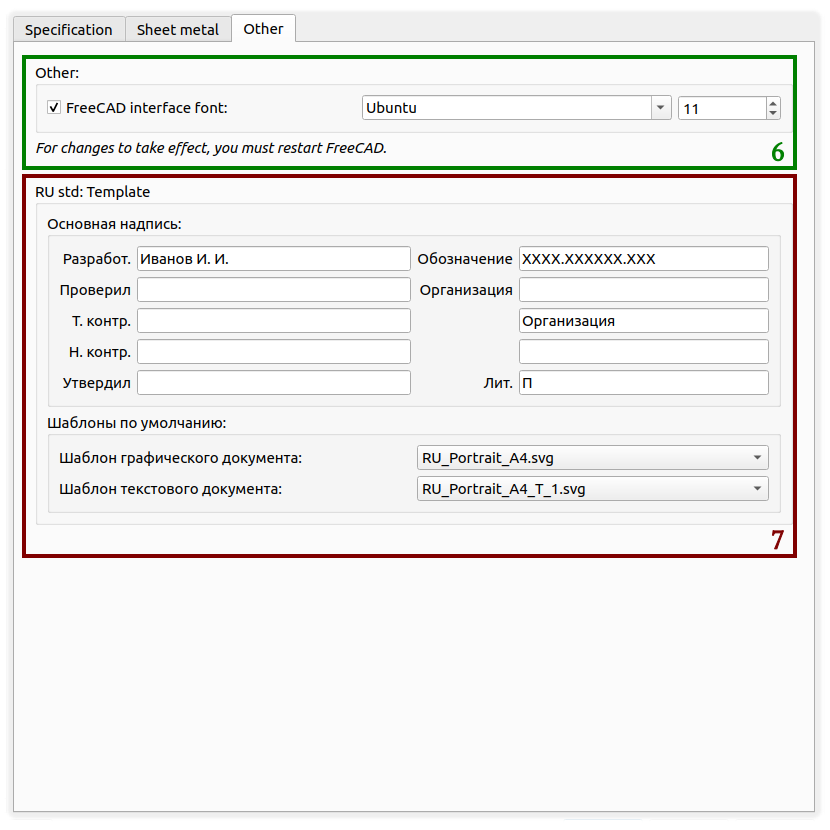
\includegraphics[width=0.9\textwidth]{img/pref_other.png}
	\caption{Дополнительные параметры}
	\label{sec:pref_other}
\end{figure}

\subsection{Область 6 -- Параметры шрифта интерфейса FreeCAD.}
В этой области можно указать необходимость подмены стандартного шрифта программы и его параметры.

\subsection{Область 7 -- Параметры для шаблонов стандарта ЕСКД и СПДС.}
В этой области можно указать значения для автоматического заполнения штампов при \hyperref[sec:8]{создании чертежей на основе шаблона} и автоматической генерации спецификации на основе модели. В качестве первого листа спецификации будет выбран шаблон указанный в соответствующем поле (шаблон текстового документа).

Все шаблоны находятся в директории -- \verb|addFC/repo/add/stdRU/tpl|

Для их корректного отображения вам \textbf{потребуется\\установить шрифт} -- \verb|addFC/repo/add/stdRU/GOST-2.304.81-A-Slanted.ttf|\\

% section end
\pagebreak




\section{Наполнение объекта свойствами}

Для добавления свойств необходимо выделить один или несколько объектов и воспользоваться командой \hyperref[sec:5]{Add Properties} на панели инструментов.

\begin{figure}[htp]
	\centering
	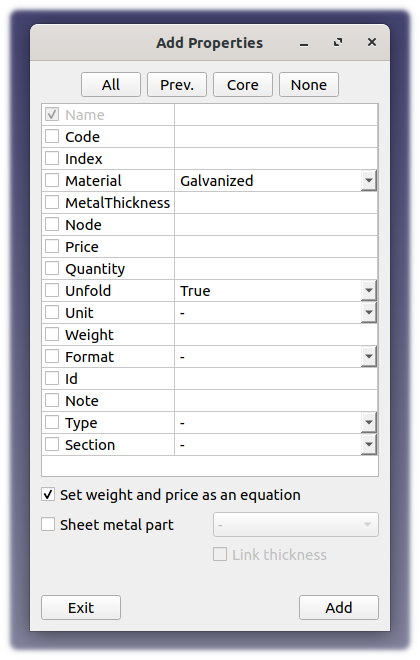
\includegraphics[scale=1]{img/properties_add.png}
	\caption{Интерфейс команды \textbf{Add Properties}}
	\label{sec:properties_add}
\end{figure}

В интерфейсе команды виден весь список доступных пользовательских свойств. Необходимо отметить нужные и нажать \textbf{Add}.\\

Кнопки \textbf{All}, \textbf{Core}, \textbf{None} -- выбрать все свойства, только основные и очистить выбор,\\соответственно.\\

Флажок \textbf{Sheet metal part} отметит все необходимые свойства для детали из листового металла, позволит выбрать тип материала и при желании связать свойство \textbf{MetalThickness} с параметрами толщины объекта. Дополнительно элементу будет присвоена масса и цвет на основе параметров указанных в настройках -- \hyperref[sec:pref_sm]{изображение 6: область 1}.\\

Примечание: В процессе присвоения имени (Name) и индекса (Index) программа пробует угадать значения свойств на основе наименования (Label) объекта.

Для автоматического заполнения этих свойств шаблон наименования должен соответствовать: \textbf{«Index. Name - Copy»} или \textbf{«Index - Name - Copy»}. В случае соответствия шаблону значения будут корректно заполнены, пример -- \hyperref[sec:properties]{изображение 5}.

% section end
\pagebreak




\section{Спецификация материалов (BOM)}

Для формирования и работы со спецификацией необходимо воспользоваться командой\\\hyperref[sec:4]{Specification} на панели инструментов. На основе пользовательских свойств программа сформирует спецификацию для любой модели (сборки), рассмотрим пример из состава верстака:

\begin{figure}[htp]
	\centering
	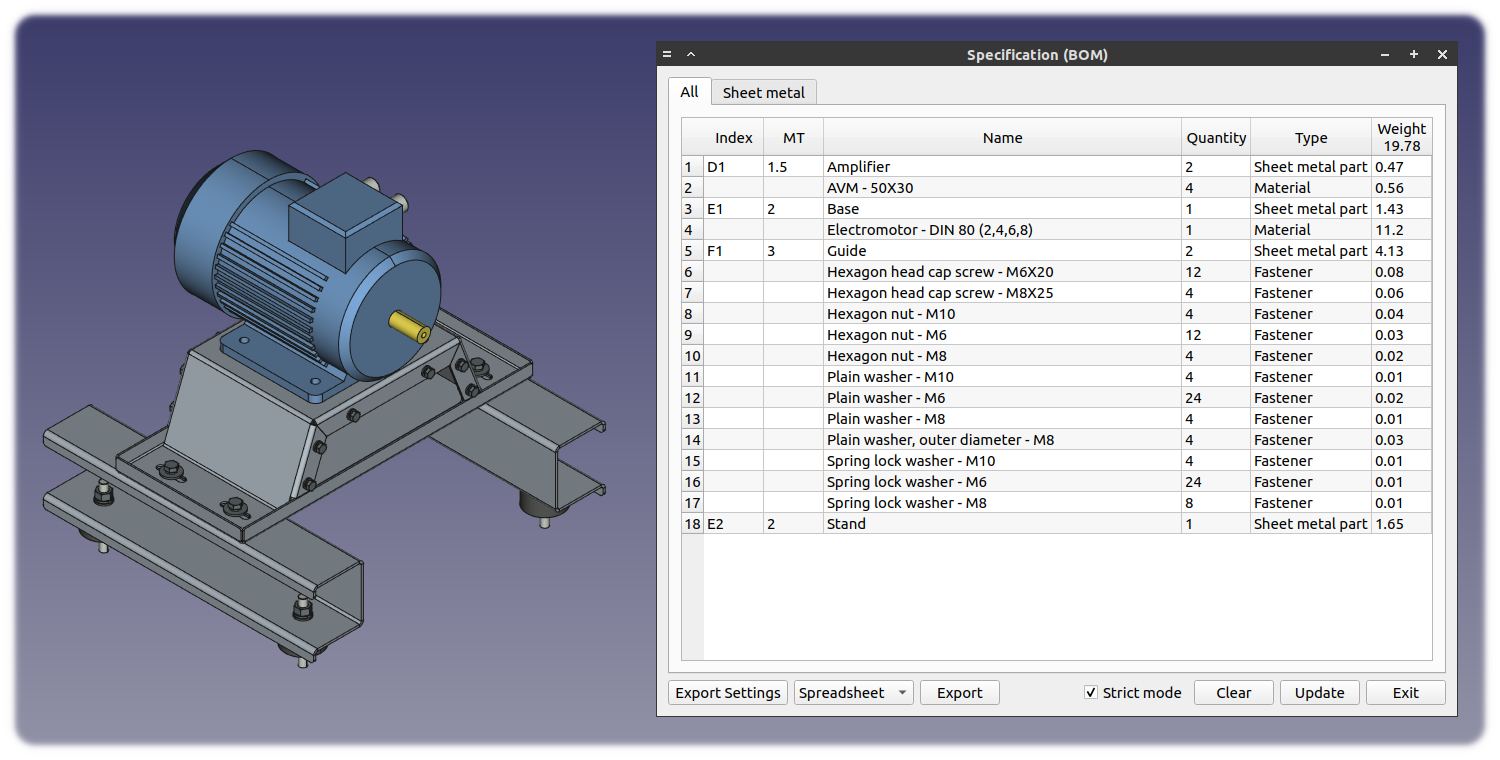
\includegraphics[width=1\textwidth]{img/specification_all.png}
	\caption{Спецификация, общая}
	\label{sec:specification_all}
\end{figure}

\begin{figure}[htp]
	\centering
	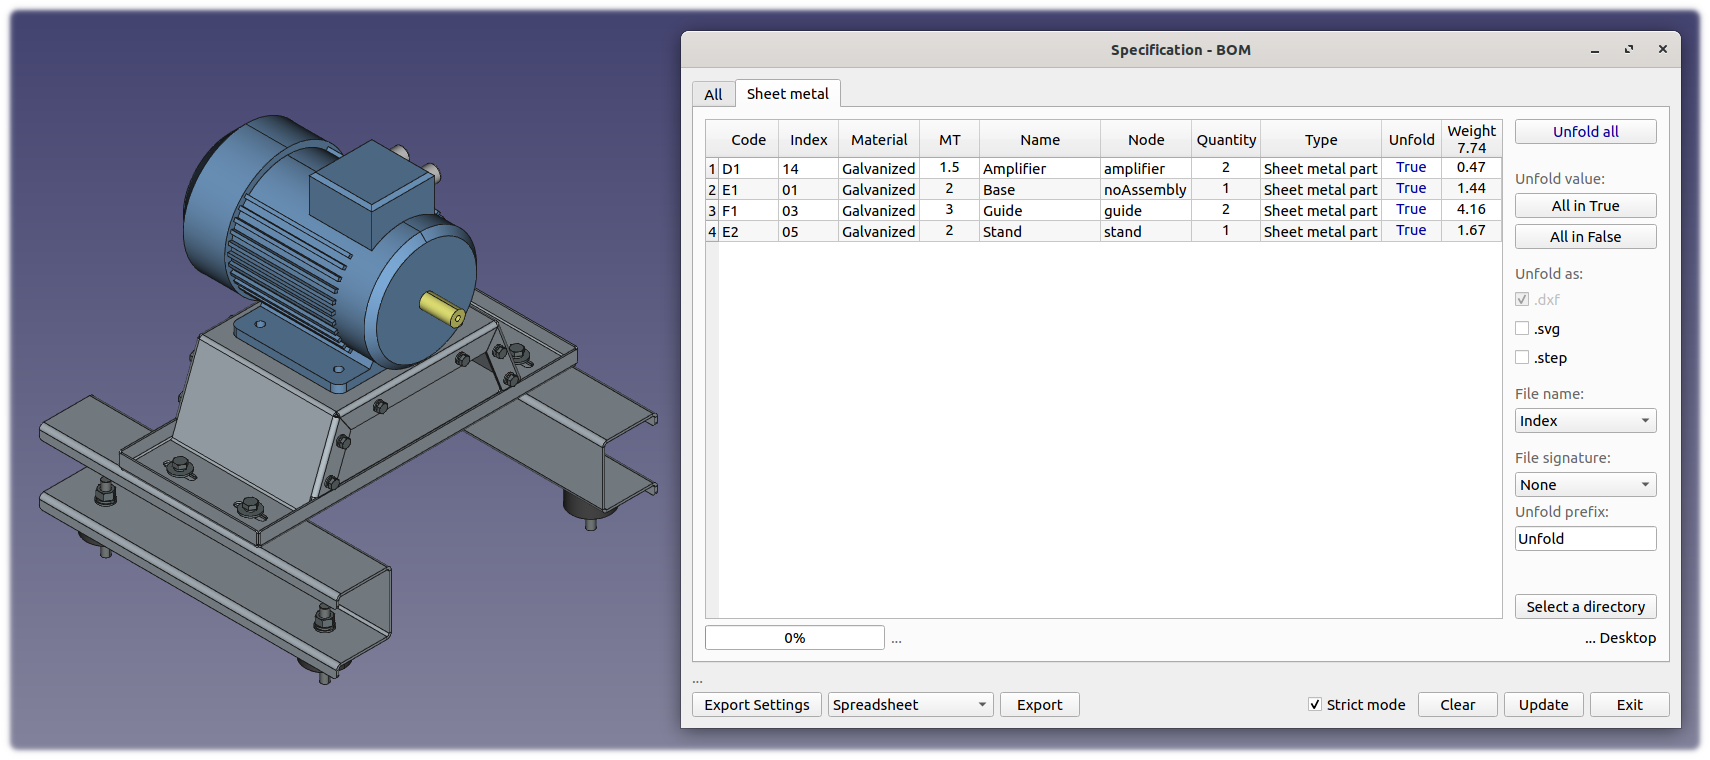
\includegraphics[width=1\textwidth]{img/specification_sm.png}
	\caption{Спецификация, листовой металл}
	\label{sec:specification_sm}
\end{figure}

\pagebreak

Интерфейс спецификации содержит две вкладки:
\begin{itemize}
	\item \textbf{All} -- все объекты.
	\item \textbf{Sheet metal} -- объекты из листового металла.
\end{itemize}

Опция \textbf{Strict mode} -- если флажок снят программа будет обрабатывать все пользовательские свойства находящиеся в вашей группе -- \hyperref[sec:pref_specification]{изображение 4: область 1}, а не только указанные в таблице (область 2).\\

На вкладке \hyperref[sec:specification_all]{общей спецификации} расположены две кнопки:
\begin{itemize}
	\item \textbf{Indexing elements} -- автоматическое проставление позиций (Index) для всех учтённых в спецификации элементов.
	\item \textbf{Update enumerations} -- обновление в объектах модели свойств содержащих списки заранее заданных значений. Полезно после добавлении новый значений в настройках.
\end{itemize}

Далее мы рассмотрим объекты из листового металла -- на \hyperref[sec:specification_sm]{данной вкладке} расположены функции для их пакетной обработки. Производственный процесс таких деталей в большинстве случаев потребует два элемента:
\begin{itemize}
	\item Заготовка (развёртка) -- плоский вид объекта для нестинга и обработки на станках.
	\item Деталь в 3D формате (step) -- для гибки листового металла.
\end{itemize}

Все детали из сформированного на основе модели (сборки) списка, в зависимости от значения свойства \textbf{Unfold}, могут быть обработаны и экспортированы во внешние файлы, такие как dxf, svg (развёртки) и step (3D).\\

\textbf{Select a directory} -- позволяет выбрать директорию для сохранения результатов работы (значение по умолчанию -- рабочий стол пользователя).\\

\textbf{Unfold prefix} -- имя директории в которую будут сохранены файлы, а также вариант для подписи детали.\\

\textbf{File signature} -- список вариантов подписи детали. Подпись -- это текст в файле, внутри контура детали, который может быть полезен при нестинге. На данный момент функция доступна только для формата dxf. При значение \textbf{None} подпись отключена.\\

\textbf{File Name} -- шаблон по которому будут названы файлы, например для детали \textbf{«E2 - Stand»} (\hyperref[sec:properties]{изображение 5}) варианты имени будут следующими:
\begin{itemize}
	\item \textbf{Name} = Stand (1).dxf
	\item \textbf{Code} = E2 (1).dxf
	\item \textbf{Index} = 05 (1).dxf
	\item \textbf{Code + Name} = (E2) Stand (1).dxf
	\item \textbf{Index + Name} = (05) Stand (1).dxf
\end{itemize}

Цифра в скобках, в конце имени -- это номер экземпляра (копии), если в сборке две или более одинаковых детали они будут сохранены в отдельные файлы.\\

После выбора нужных опций и параметров можно нажать кнопку \textbf{Unfold} и программа сохранит все полученные данные по указанному пути. Процесс работы можно наблюдать в индикаторе прогресса и во FreeCAD, на панели отчёта (report view).\\

Важно: файлы деталей будут размещены в дополнительных директориях, имена которых соответствуют псевдониму (Alias) толщины стали -- \hyperref[sec:pref_sm]{изображение 6: область 2}.

% section end
\pagebreak




\section{Экспорт спецификации}

Программа может экспортировать спецификацию модели (сборки) для последующего просмотра, редактирования или иного использования, доступные форматы:

\begin{itemize}
	\item \href{https://wiki.freecad.org/Spreadsheet_Workbench}{\textbf{Spreadsheet}} -- электронная таблица FreeCAD.
	\item \href{https://ru.wikipedia.org/wiki/JSON}{\textbf{json}} --  текстовый формат обмена данными, самый подходящий вариант для последующей автоматизации.
	\item \href{https://ru.wikipedia.org/wiki/CSV}{\textbf{csv}} -- представление базы данных.
	\item \textbf{RU std: Spreadsheet} -- создание электронной таблицы со спецификацией в формате ЕСКД.
	\item \textbf{RU std: TechDraw} -- выгрузка спецификации в оформлении текстового документа ЕСКД.\\
\end{itemize}

\begin{flushleft}Для начала рассмотрим параметры экспорта, кнопка \textbf{Export Settings}.\end{flushleft}

\begin{figure}[htp]
	\centering
	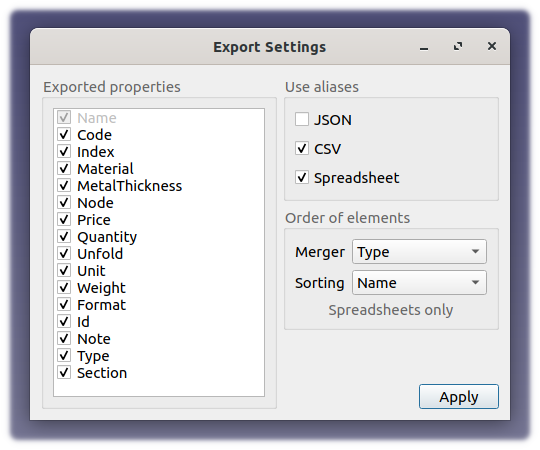
\includegraphics[scale=1]{img/specification_export.png}
	\caption{Параметры экспорта спецификации}
	\label{sec:specification_export}
\end{figure}

В левой части интерфейса можно выбрать свойства которые будут экспортированны.\\

В области \textbf{Use aliases} нужно отметить форматы в которых будут использоваться псевдонимы, как замена имени (Title) свойства.\\

\pagebreak

В области \textbf{Order of elements} нужно указать свойства для группировки и сортировки объектов:

\begin{itemize}
	\item \textbf{Merger} -- свойство по значению которого элементы будут сгруппированы, самое подходящее -- тип объекта (Type), например вывести сначала все метизы, потом материалы, следом -- детали.
	\item \textbf{Sorting} -- свойство по значению которого объекты будут сортированы внутри группы (Merger), самое логичное -- сортировать по индексу (Index) или имени (Name).
\end{itemize}

Примечание: в вариантах выгрузки спецификации по правилам ЕСКД элементы будут\\сгруппированы по значениям свойства \textbf{Section}, в соответсвии со стандартами оформления.\\

Выберете необходимые опции, подходящий формат и нажмите кнопку \textbf{Export}.

\begin{figure}[htp]
	\centering
	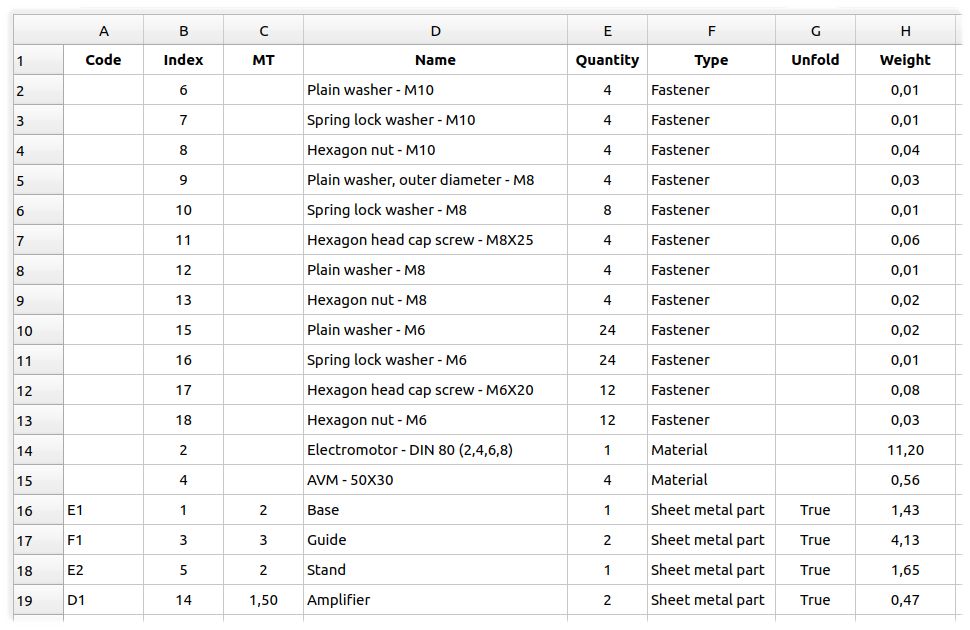
\includegraphics[width=1\textwidth]{img/specification_result.png}
	\caption{Результат экспорта спецификации}
	\label{sec:specification_result}
\end{figure}

\begin{figure}[htp]
	\centering
	
\includegraphics[width=1\textwidth]{img/specification_result_ru.png}
	\caption{Результат экспорта спецификации по правилам ЕСКД}
	\label{sec:specification_result}
\end{figure}

% section end
\pagebreak




\section{Управление моделью}

На панели задач доступна команда \hyperref[sec:3]{Model Control} назначение которой -- запустить управляющую программу для \textbf{параметрической} модели.\\

В своей работе я убедился, что не одна из существующих (для FreeCAD) систем сборок в комплексе с таблицами и уравнениями не способна дать таких возможностей, которые доступны из программного кода.

Своим параметрический моделям я пишу управляющие файлы и интерфейсы, вызывать которые удобно одной командой, для этого рядом с основным файлом модели (сборки) должны находиться два файла названные аналогично основному.\\

В образцах поставляемых вместе с верстаком доступен простой пример параметрической модели для изучения -- \verb|addFC/repo/example|

\begin{figure}[htp]
	\centering
	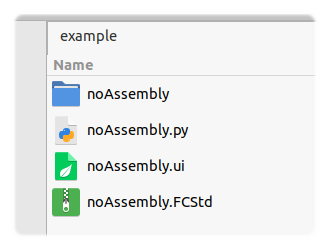
\includegraphics[scale=1]{img/example.png}
	\caption{Файлы параметрической модели}
	\label{sec:example}
	\end{figure}

\begin{itemize}
	\item \textbf{.FCStd} -- основной файл модели -- сборка.
	\item \textbf{.ui} -- интерфейс пользователя -- Qt.
	\item \textbf{.py} -- управляющий код -- Python.
	\item \textbf{noAssembly} -- директория с дополнительными файлами.
\end{itemize}

\pagebreak

\begin{flushleft}Открыв основной файл, командой \hyperref[sec:3]{Model Control} можно вызвать его управляющую программу:\end{flushleft}

\begin{figure}[htp]
	\centering
	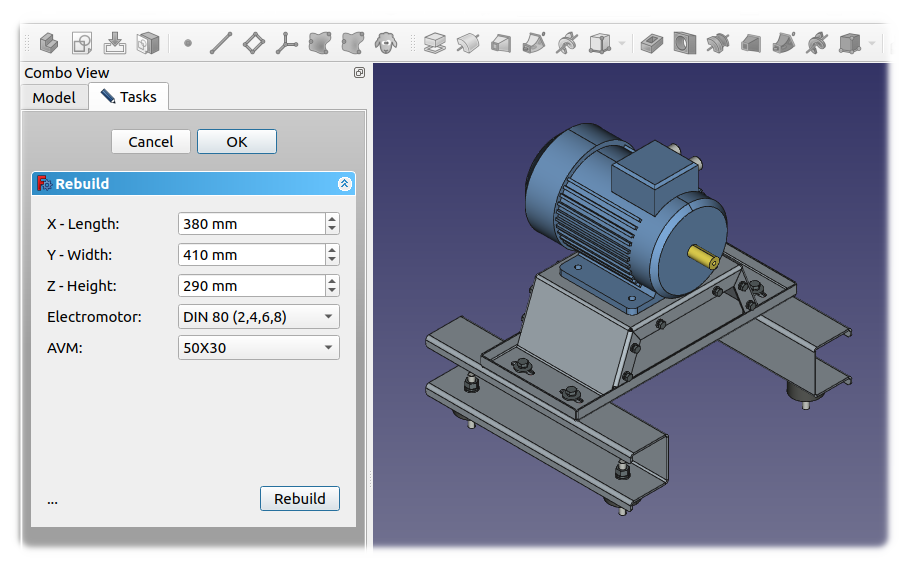
\includegraphics[width=1\textwidth]{img/example_mc.png}
	\caption{Интерфейс управления параметрической моделью}
	\label{sec:example_mc}
\end{figure}

Для удобства графический интерфейс пользователя встроен в боковую панель FreeCAD, задав в нём необходимые параметры и выбрав из списков комплектующие нажмите кнопку \textbf{Rebuild} -- модель перестроится.

% section end
\pagebreak




\section{Создание трубопровода по координатам}
Продолжение следует ...
% section end


\section{Вид с разнесёнными частями}
Продолжение следует ...
% section end




\end{document}